\documentclass[12pt, letterpaper]{article}
\usepackage[colorlinks=true,linkcolor=black,citecolor=blue,filecolor=cyan,pagecolor=blue]{hyperref} 
\usepackage[toc,style=altlistgroup,hyperfirst=false]{glossaries}
\usepackage[utf8]{inputenc} %para poder escribir símbolos no anglosajones 
\usepackage[spanish, mexico]{babel} %Escribir en español (acentos)
\usepackage[T1]{fontenc}
\usepackage{amssymb}
\usepackage{mathtools}
\usepackage[usenames]{color}
\usepackage{float}
\usepackage{graphicx}  %%para las imagenes
\usepackage{cite} % para contraer referencias
\usepackage{multicol}
\usepackage{multirow}
\usepackage{bm}
\usepackage{bbm}
\usepackage[left=2.5cm,top=2.5cm,right=2.5cm,bottom=2.5cm]{geometry}
\parindent=5mm
\graphicspath{{images/}}
\usepackage{etoolbox}
\let\bbordermatrix\bordermatrix
\patchcmd{\bbordermatrix}{8.75}{4.75}{}{}
\patchcmd{\bbordermatrix}{\left(}{\left[}{}{}
\patchcmd{\bbordermatrix}{\right)}{\right]}{}{}
%%%%glosario
\makeindex
%\makeglossaries
%\input{./glosario.tex}

%%%%%%%%%%%%%%%%%%%%%%%%%%%%%%%%%%%%%%%%%%%%%%%%%%%%%%%%%%%%%%%%%%%%%%%%%%%%%
%%NOTA IMPORTANTE:
%%Para relacionar el glosario.tex con este archivo
%%Es necesario abrir la terminal (Simbolo del sistema en windows)
%%Ir a la carpeta contenedora y escribir el siguiente comando:
%%makeindex -s PROYECTO_final.ist -t PROYECTO_final.glg -o PROYECTO_final.gls PROYECTO_final.glo
%%%%%%%%%%%%%%%%%%%%%%%%%%%%%%%%%%%%%%%%%%%%%%%%%%%%%%%%%%%%%%%%%%%%%%%%%%%%%

%%%% inicio del documento
\begin{document}

\thispagestyle{empty}

%%%%%%% portada

\thispagestyle{empty}

\begin{minipage}[c][0.1\textheight][c]{0.2\textwidth}
\begin{center}
    
\includegraphics[width=4cm, height=4cm]{cimat}
\end{center}
\end{minipage}
\begin{minipage}[c][0.1\textheight][t]{0.8\textwidth}
\begin{center}
    {\hspace{2cm}\scshape Centro de Investigación en Matemáticas}
    \vspace{-.5cm}
\end{center}
\hspace*{1.0cm} \rule[0mm]{0.9\textwidth}{0.8mm}
\hspace*{1.17cm}   \rule[4mm]{0.9\textwidth}{0.1mm}
    \vspace{-1cm}
\begin{center}
    { \hspace{2cm}\scshape  Unidad Monterrey}
\end{center}
\end{minipage}

\begin{minipage}[c][0.6\textheight][t]{0.2\textwidth}
\begin{center}
\hskip2pt
\vrule width2.5pt height10cm
        \hskip1mm
        \vrule width1pt height10cm \\ \vspace{2cm}
        
\includegraphics[height=4.5cm]{mty}
        \end{center}
\end{minipage}
\begin{minipage}[c][0.9\textheight][t]{0.65\textwidth}
  \begin{center}

	
    \vspace{3.2cm}
    
%%%% TITULO EN PORTADA

  \scshape Proyecto No. 1.\\ \normalsize
  
  \vspace{2cm}  
  
    
            
    Métodos multivariados de Análisis de Datos\\
    \vspace{1cm}   
    Análisis de nutrientes en pizzas.\\
    \vspace{1cm}   
    \vspace{1cm}   
    Ricardo Cruz Sánchez\\
    Rolando Corona Jiménez
    \vspace{.5cm}   
  \end{center}
  
\end{minipage}

%TABLA DE INDICES
\pagebreak
\tableofcontents

\cleardoublepage
%INTRODUCCIÓN
\pagebreak
\section{Introducción.}
La bromatología es la ciencia encargada del análisis de los nutrientes contenidos en los alimentos. Los estudios relacionados con esta disciplina cobran importancia al considerar que existen cantidades recomendadas en la ingesta diaria de cualquier individuo y el incremento o decremento de las cantidades repercute directamente en la salud del la persona.\\

Las porciones de nutrientes que posee cierto alimento en particular, se determinan a través de diversas pruebas de laboratorio, las cuales buscan ser lo más precisas y por lo general reportan los nutrientes contenidos en 100 gramos del alimento en cuestión.\\

Los alimentos considerados como \emph{comida rápida} suelen tener cantidades elevadas en los nutrientes, por lo que la ingesta de este tipo de alimentos suele sobrepasar o aportar considerablemente a los límites recomendados.\\

Particularmente, la pizza, tiende a ser uno de los alimentos con los cuales se sobrepasan los límites de nutrientes recomendados. Esto, principalmente, se debe a que es una mezcla de ingredientes cuya aportación nutrimental es elevada, a saber, harina, tomate, queso y carne.\\
 
En el presente trabajo, se considera una base de datos relativa a las pruebas nutrimentales realizadas en distintas pizzas y con base a estos datos se pretende realizar un análisis multivariado.\\

El documento se divide en 4 secciones, la primera de ellas realiza un análisis exploratorio de los datos, donde se presentan las variables y resumen de datos a través medidas en forma de gráficas. Esta exploración se hace con el fin de conocer mejor las variables y tener una idea a priori de los resultados esperados. Posteriormete, la segunda sección implementa los modelos de reducción de dimensiones, enfocados en trabajar en un espacio que permita una mejor visualización de los datos. La siguiente sección, presenta los modelos de clasificación, con los que se espera asignar una categoría a cada tupla de datos, considerados como variables predictivas. Por último, la última sección resume los resultados obtenidos y plantea las mejoras que se pueden realizar a este tipo de trabajos.\\

El documento, así como los códigos, datos, gráficas y resultados de este trabajo se encuentran en el siguiente repositorio:
\url{https://github.com/rolandocj/proyecto-pizzas/tree/develop}
\pagebreak

\section{Análisis exploratorio.}
La base de datos, \emph{pizzas.xls}, proporcionada para el desarrollo de este proyecto consta de 9 variables y 379 registros. El significado de cada una de las variables se explica a continuación.

\begin{itemize}
\item \textbf{Ident:} Variable tipo numérica, la cual corresponde a un identificador para cada pizza.
\item \textbf{HUMED:} Variable tipo numérica que indica el porcentaje de humedad contenido en la pizza.
\item \textbf{PROTE:} Variable tipo numérica que indica la cantidad de gramos de proteina contenida en 100g de pizza.
\item \textbf{GRASA:} Variable tipo numérica que indica la cantidad de gramos de grasa contenida en 100g de pizza.
\item \textbf{CENIZA:} Variable tipo numérica que indica la cantidad de gramos de ceniza contenida en 100g de pizza.
\item \textbf{SODIO:} Variable tipo numérica que indica la cantidad de gramos de sodio contenida en 100g de pizza.
\item \textbf{CARBO:} Variable tipo numérica que indica la cantidad de gramos de carbohidratos contenida en 100g de pizza.
\item \textbf{CALOR:} Variable tipo numérica que indica la cantidad de calorias contenida en 100g de pizza.
\item \textbf{MARCA:} Varibale tipo string, la cual indica la marca que fabrico la pizza. Es una variable categórica.
\end{itemize}

Conociendo solo esto, una duda natural sería ¿Existe algún comportamiento significativo por marca? ya que MARCA es la única variable categórica. Para esto, primero se analizará dicha variable. En la figura \ref{i1}, se muestra como la muestras, si no están balanceadas perfectamente, casi todas entran en el mismo rango de observaciones, variando desde 30 hasta 36 observaciones por marca.\\

\begin{figure}[h]
\centering
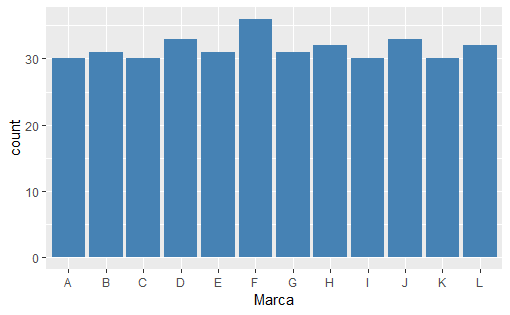
\includegraphics[scale=1]{images/marca.png} 
\label{i1}
\caption{Conteo de registros por marca}
\end{figure}

Se continua con el análisis del resto de las variables y empiricamente se puede considerar que la variable Ident no aportará mucho considerando comportamientos de acuerdo a marca. La figura \ref{i2} muestra el scatterplot de esta variable considerando el etiquetado por marca. Lo rescatable de esta gráfica son dos saltos que se presentan, las cuales sugieren prestar atención en las marcas donde se presentan estos saltos.\\

\begin{figure}[h]
\centering
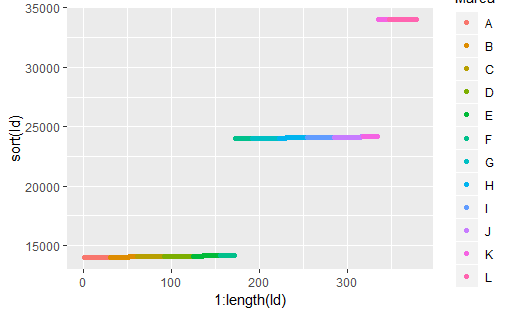
\includegraphics[scale=1]{images/ident.png} 
\label{i2}
\caption{Comportamiento de la variable Ident de acuerdo a la marca}
\end{figure}

A partir de este punto, las variables restantes son características del alimento en cuestión. Cabe resaltar que cada una de ellas se obtiene a través de diversos procesos químicos los cuales son importantes de especificar, ya que, para una sola característica pueden existir diversas metodologías para su medición y cada una de ellas posee su error de medición o simplemente su eficiencia se enfoca en cierto tipo de alimentos, prepaciones y/o presentaciones.\\

Sin embargo, para esta base de datos no fue posible recolectar este tipo de información. Por lo tanto se procede considerando que se implemento la medición adecuada con una formula estandar para todas las pizzas que permita la comparación y la ejecución de los procesos en ambientes similares.\\

Para cada una de las variables, se selecciono el gráfico \emph{boxplot} como manera idonea de resumir el comportamiento. Esto debido a que el boxplot contiene varias medidas de interés y gráficamente al comparar dos o más se pueden distinguir comportamientos visuales importantes.\\

Comenzado con la variable HUMED, en la figura \ref{i3} se aprecia que existe un comportamiento homogeneo de humedad dentro de cada marca, no así entre marcas, pues se pueden distinguir 3 grupos de acuerdo al nivel de humedad presentado.\\

\begin{figure}[h]
\centering
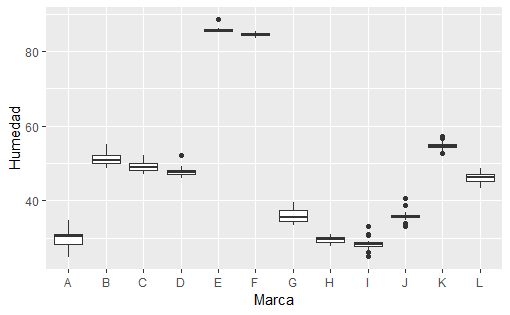
\includegraphics[scale=1]{images/humed.png} 
\label{i3}
\caption{Comportamiento de la variable Humed de acuerdo a la marca}
\end{figure}

Para la variable PROTE, se aprecia un comportamiento similar, en la figura \ref{i4} se muestra un comportamiento elevado en las primeras 4 marcas en comparación al resto.\\

\begin{figure}[h]
\centering
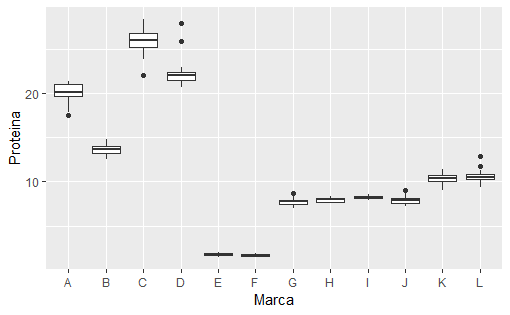
\includegraphics[scale=1]{images/prote.png} 
\label{i4}
\caption{Comportamiento de la variable Prote de acuerdo a la marca}
\end{figure}

Para la variable GRASA, la figura \ref{i5} muestra como existen 2 grupos y particularmente la marca H presenta observaciones en los dos grupos marcados.\\

\begin{figure}[h]
\centering
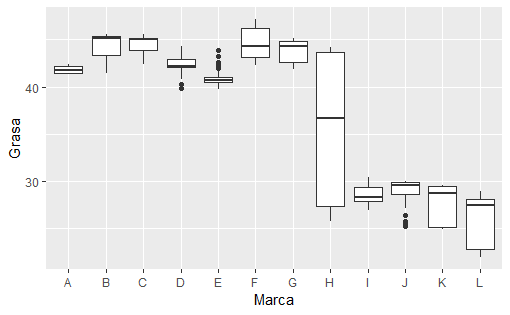
\includegraphics[scale=1]{images/grasa.png} 
\label{i5}
\caption{Comportamiento de la variable Grasa de acuerdo a la marca}
\end{figure}

Para la variable CENIZ, la figura \ref{i6} muestra un efecto similar al de proteinas, pues las primeras 4 marcas presentan niveles elevados, lo cual es de interés, pues al menos en México, existen normas las cuales regulan que el nivel de sodio no exceda 3 g por cada 100 g del alimento. Sin embargo, no se posee información de la procedencia de la base de datos.\\

\begin{figure}[h]
\centering
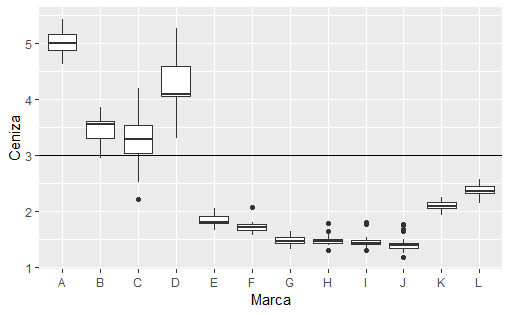
\includegraphics[scale=1]{images/ceniz.png} 
\label{i6}
\caption{Comportamiento de la variable CENIZ de acuerdo a la marca}
\end{figure}

La variable SODIO, resumida en la figura \ref{i7}, muestra niveles altos de sodio para la marca A y un comportamiento homogeneo en el resto de las marcas. En México, una rebanada de pizza mediana oscila entre los 75.7 y 100.7 g en promedio y el límite recomendado de sodio para una persona mayor de 19 años es de 2400mg, esto quiere decir que las pizzas de la marca A, contienen más de la mitad del sodio recomendado diario en una sola rebanada.\\

El comportamiento similar entre proteinas y sodio podría ser explicado por sus ingredientes si es que no todas las pizzas tienen una formula estandar, pues las pizzas que tienen más proteina podría ser explicado por la presencia de productos carnicos y tendría el efecto similar en el sodio.

\begin{figure}[h]
\centering
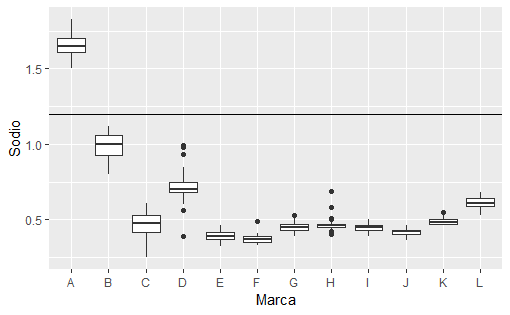
\includegraphics[scale=1]{images/sodio.png} 
\label{i7}
\caption{Comportamiento de la variable sodio de acuerdo a la marca}
\end{figure}

Para la variable CARBO, la figura \ref{i8} presenta 3 grupos separados por el nivel de carbohidratos.\\

\begin{figure}[h]
\centering
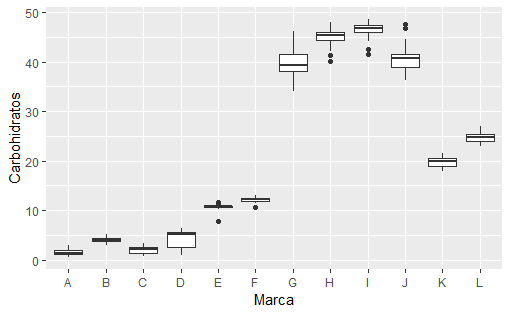
\includegraphics[scale=1]{images/carbo.png} 
\label{i8}
\caption{Comportamiento de la variable Carbo de acuerdo a la marca}
\end{figure}

Para la variable CALOR, la figura \ref{i9} muestra 3 grupos de acuerdo al nivel de calorias contenidas.\\

\begin{figure}[h]
\centering
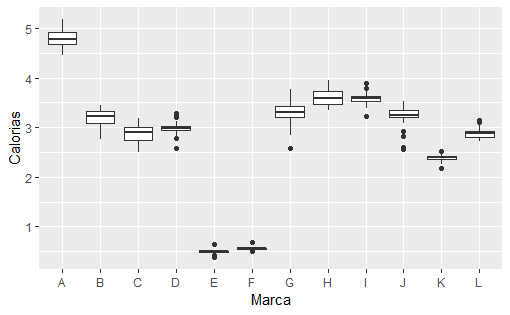
\includegraphics[scale=1]{images/calor.png} 
\label{i9}
\caption{Comportamiento de la variable Calor de acuerdo a la marca}
\end{figure}

Empiricamente, un nutriologo puede considerar que los principales nutrientes de un alimento son carbohidratos, grasas y proteinas. La suma del gramaje de cada una de estas componentes debe ser muy cercano al total de masa. En nuestro caso, deberían sumar alguna cantidad proxima a 100g. La figura \ref{i10} muestra que solo 2 marcas, G y H, tienen cantidades cercanas a 100g, por lo tanto, debe existir algo más en la composición cuyo gramaje sea significativo, ejemplos de esto, pueden ser fibras crudas contenidas en harinas y verduras.\\

\begin{figure}[h]
\centering
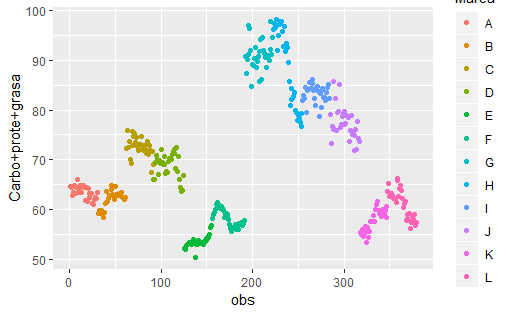
\includegraphics[scale=1]{images/pgc.png} 
\label{i10}
\caption{Grasa+Proteina+Carbohidratos para cada observación}
\end{figure}

En la teoría de la bromatología, existen aproximaciones que se satisfacen con buena precisión entre las calorías y algunos nutrientes. Las aproximaciones se muestran a continuación:\\

\begin{itemize}
\item una caloría por cada 6 gramos carbohidratos
\item una caloría por cada 9 gramos de grasas
\item una caloría por cada 4 gramos de proteina
\end{itemize}

Si los datos se calcularon de manera correcta, la diferencia entre las calorías registradas debería ser próximo al nutriente dividido por su respectivo factor.\\

Los cálculos de las aproximaciones arrojaron los siguientes errores para cada uno de los nutrientes\\

\begin{table}[htbp]
\begin{center}
\begin{tabular}{|l|l|}
\hline
Nutriente&Error promedio\\ \hline\hline
Carbohidratos&1.37\\ \hline
Grasas&0.68\\ \hline
Proteina&0.04\\ \hline
\end{tabular}
\end{center}
\end{table}

Por último, se presenta un gráfico de correlación entre las características de los alimentos. La figura \ref{i11} muestra, al menos 4 patrones importantes, a saber, Humedad-calorias, Proteina-ceniza, Ceniza-sodio y Ceniza-carbohidratos\\

La relación entre humedad y calorías, tal vez corresponda a la presencia del fosfato, pues la presencia de fosfato modifica el valor de estas dos variables y se encuentra en alimentos como el queso y carnes.\\

La alta correlación entre Proteinas y cenizas puede ser explicado por la presencia de queso, pues es un alimento el cual es fuente de proteinas y minerales.\\

En el caso de la alta correlación entre sodio y cenizas, puede ser explicado por la presencia de tomate, ya que, este alimento eleva el valor de ambas variables.\\

\begin{figure}[h]
\centering
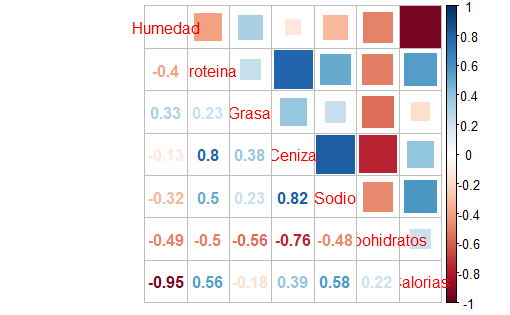
\includegraphics[scale=1]{images/corr.png} 
\label{i11}
\caption{Correlación de las variables.}
\end{figure}


\pagebreak
\restoregeometry 
\section{Modelos de reducción de dimensiones.}

\subsection{Análisis de componentes principales (PCA)}

Al hacer el análisis de componentes principales a los datos se obtuvieron las siguientes cargas en las primeras dos componentes. La varianza acumulada en las primeras dos componentes es del $83.59 \%$ y se considera suficiente para el análisis.
Como se puede observar la primera componente está asociada con la ceniza, el sodio y la proteína, mientras que la segunda se asocia con la humedad, los carbohidratos y las calorías.
Las componentes principales se obtuvieron usando la función \textsf{prcomp} de R con los datos normalizados, la normalización no afectó drásticamente la representación gráfica, sin embargo, permitió observar de forma más clara las relaciones entre las variables ya mencionadas.


\begin{table}[ht]
\centering
\begin{tabular}{rrr}
  \hline
 & PC1 & PC2 \\ 
  \hline
Humedad & 0.21 & 0.58 \\ 
  Proteina & -0.47 & -0.03 \\ 
  Grasa & -0.19 & 0.41 \\ 
  Ceniza & -0.51 & 0.15 \\ 
  Sodio & -0.47 & -0.02 \\ 
  Carbohidratos & 0.32 & -0.49 \\ 
  Calorias & -0.34 & -0.48 \\ 
  Varianza acumulada & 48.64 \% &  83.59 \% \\ 
\end{tabular}
	\label{tabla:pesos_PCA}
	\caption{Pesos asociados a las primeras dos componentes principales.}
\end{table}


\begin{figure}[h]
\centering
	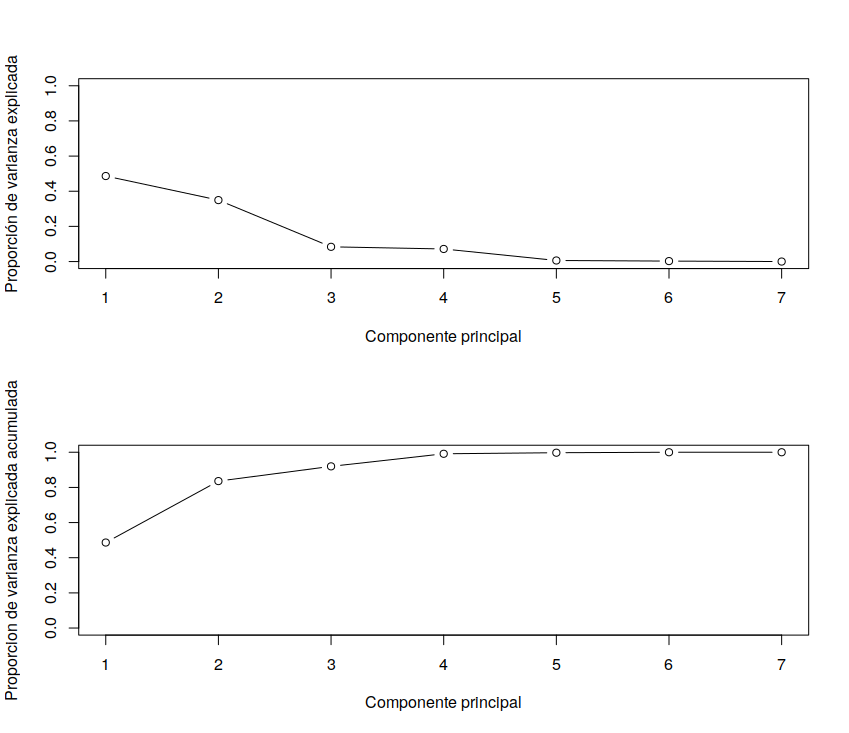
\includegraphics[scale=.5]{images/varPCA.png} 
	\label{i_var_PCA}
	\caption{Varianza explicada por las componentes principales}
\end{figure}

\subsubsection{Representación gráfica (biplot)}

La figura  \ref{i_biplot_PCA} muestra la representación en las primeras dos componentes principales de los datos, en ella se aprecia una clara separación entre algunos grupos de pizzas, específicamente, la marca A se distingue por tener altos niveles de sodio y proteina, las marcas B, C y D se caracterizan por un alto nivel de ceniza, E y F por tener altos valores de humedad, finalmente el resto de marcas (G, H, I, J, K y L) se distinguen por su alto contenido en carbohidratos. 
También el biplot muestra la alta colinealidad existente entre las variables sodio y proteina, y sugiere un contraste entre la variables grasa y carbohidratos.


\begin{figure}[h]
\centering
	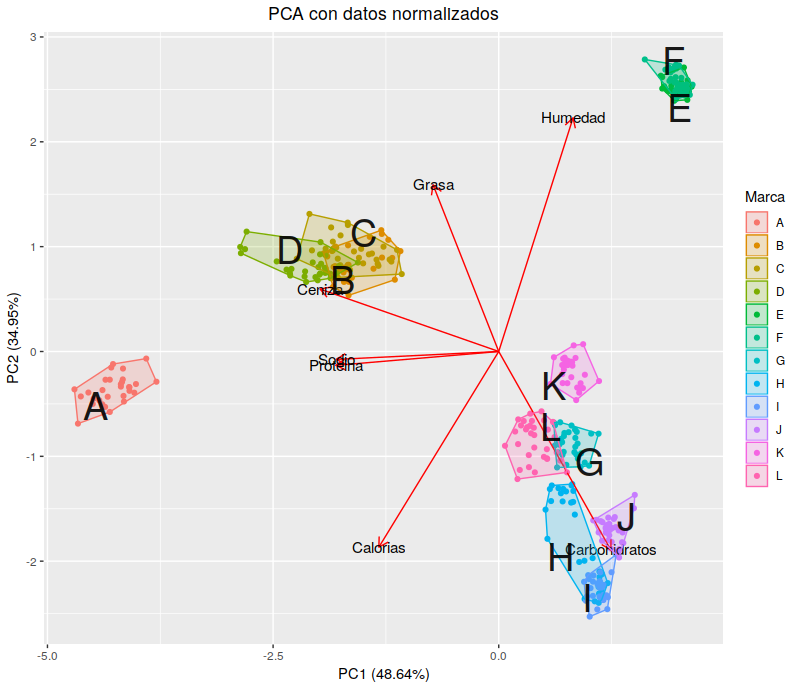
\includegraphics[scale=.75]{images/biplotPCA.png} 
	\label{i_biplot_PCA}
	\caption{Biplot PCA}
\end{figure}


\restoregeometry 
\subsection{Análisis de factores}

Se realizó el análisis de factores usando dos factores, esto debido a la baja dimensión del problema. Para ello se uso la función \textsf{factanal} de R, que estima los factores usando el método de máxima verosímilitud, además, se usó la rotación varimax. \\
El resumen de los resultados se muestra en la tabla \ref{tabla:factores}. El valor del estadístico de prueba $\chi^2$ (con 8 grados de libertad) para verificar la hipótesis nula que la matriz de correlación de datos puede ser representada usando dos factores es $1837.4$, obteniendo además un $p-$valor de 0, por lo que la hipótesis nula se rechaza. Este resultado puede ser explicado por el hecho de que el determinante de la matriz de correlación es cercano a cero. A pesar de ello, se puede afirmar que la aproximación a la matriz de correlación a partir de la matriz $LL' + \Psi$ es adecuada, como se muestra en la tabla \ref{tabla:aproximacion}, la diferencia entre la matriz R y $LL' + \Psi$ es mínima, considerando un redondeo a tres dígitos. Esto en conjunto con el hecho que la proporción de varianza acumulada usando dos factores es del $80.9 \%$, permite afirmar que dos factores son suficientes para la representación de los datos.

\begin{table}[ht]
\centering
\begin{tabular}{rrrrr}
  \hline
 & Factor1 & Factor2 & Varianza específica & Comunalidades \\ 
  \hline
Humedad & 0.06 & -1.00 & 0.01 & 1.00 \\ 
  Proteina & 0.76 & 0.44 & 0.23 & 0.77 \\ 
  Grasa & 0.47 & -0.30 & 0.69 & 0.31 \\ 
  Ceniza & 0.94 & 0.19 & 0.08 & 0.92 \\ 
  Sodio & 0.73 & 0.39 & 0.32 & 0.68 \\ 
  Carbohidratos & -0.90 & 0.44 & 0.01 & 1.00 \\ 
  Calorias & 0.23 & 0.97 & 0.01 & 0.99 \\     
  Proporción de Varianza  & 44 \% &  36.9 \% \\
  Varianza acumulada & 44 \% &  80.9 \% \\ 
   \hline
\end{tabular}
	\label{tabla:factores}
	\caption{Resultados del análisis factorial.}
\end{table}


\begin{table}[ht]
\centering
\begin{tabular}{rrrrrrrr}
  \hline
 & Humedad & Proteina & Grasa & Ceniza & Sodio & Carbohidratos & Calorias \\ 
  \hline
Humedad & -0.00 & -0.02 & 0.00 & -0.00 & 0.01 & -0.00 & -0.00 \\ 
  Proteina & -0.02 & 0.00 & -0.01 & -0.01 & -0.22 & -0.01 & -0.04 \\ 
  Grasa & 0.00 & -0.01 & 0.00 & -0.01 & -0.00 & -0.00 & 0.00 \\ 
  Ceniza & -0.00 & -0.01 & -0.01 & -0.00 & 0.06 & 0.00 & -0.00 \\ 
  Sodio & 0.01 & -0.22 & -0.00 & 0.06 & -0.00 & 0.01 & 0.04 \\ 
  Carbohidratos & -0.00 & -0.01 & -0.00 & 0.00 & 0.01 & -0.00 & -0.00 \\ 
  Calorias & -0.00 & -0.04 & 0.00 & -0.00 & 0.04 & -0.00 & 0.00 \\ 
   \hline
\end{tabular}
	\label{tabla:aproximacion}
	\caption{Diferencia entre R y $LL' + \Psi$, con redondeo a tres dígitos.}
\end{table}

\subsubsection{Interpretación}

El primer factor se relaciona principalmente con las variables ceniza, carbohidratos y proteina mientras que el segundo factor se asocia con la humedad y las calorías. Las varianzas específicas y las comunalidades indican que la varianza de la mayoría de las variables queda bien explicada a partir de los factores, con excepción de la variable grasa, cuya varianza específica es de $.69$.

\subsubsection{Representación gráfica (biplot)}

Para obtener una representación gráfica en dos dimensiones, se realizó la estimación de los \textit{scores} usando el método de Bartlett. El biplot resultante se muestra en la figura \ref{i_biplot_Factores}. El resultado es muy similar al obtenido usando componentes principales, pues se logran diferenciar los mismos grupos que las marcas forman de acuerdo a sus características; sin embargo, existe una pequeña diferencia y es que las marcas K y L se separan del grupo formado por las marcas G, H, I y J, para situarse más al centro de la gráfica, lo que indica que los niveles de nutrientes de las marcas K y L se situán en la media o por debajo de ella.

\begin{figure}[h]
\centering
	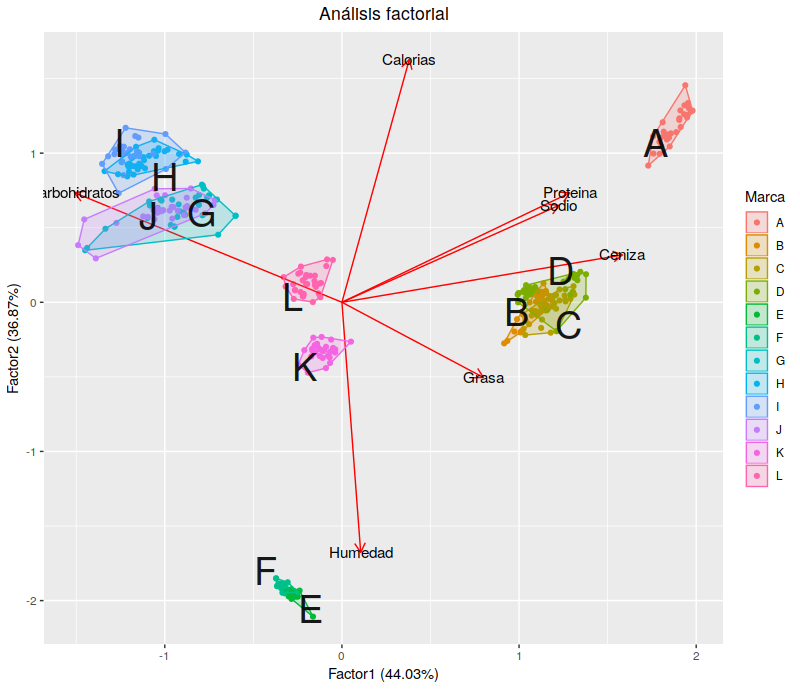
\includegraphics[scale=.75]{images/biplotFactores.png} 
	\label{i_biplot_Factores}
	\caption{Biplot usando 2 factores}
\end{figure} 
\pagebreak
\restoregeometry 
\section{Análisis por agrupación.}

Con el fin de identificar grupos con características similares de forma automática, se procedió a usar algoritmos de clustering. Específicamente, se hace clustering jerárquico completo usando la función \textsf{agnes} de la biblioteca \textsf{cluster}. 

\subsection{Elección del número de clusters}

Existen criterios para la elección de número de clusters adecuado dado un conjunto de datos, los criterios utilizados en este problema son dos:  suma de cuadrados entre clústers (wss) y el criterio de ancho de \textit{silhouette}.
En el primer caso, el criterio consiste en graficar la suma de cuadrados entre clústers para varios números de clústers y observar a partir de que número la mejora a la suma de cuadrados entre clústers es mínima. En una gráfica que compare a wss con el número de clusters, se espera que en el número óptimo se forme un \textit{codo} que indique el cumplimiento del criterio. La figura \ref{i_cluster_Elbow} muestra el resultado de calcular wss para ciertos números de clústers. A partir de observar la gráfica, se determina que una cantidad adecuada para el número de clusters usando estre criterio es $5$.


\begin{figure}[h]
\centering
	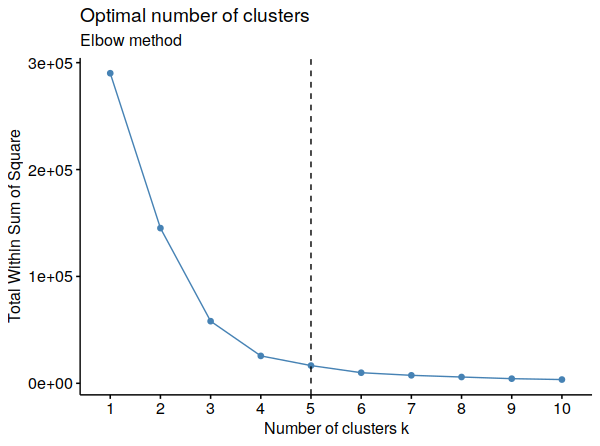
\includegraphics[scale=.5]{images/clusterElbow.png} 
	\label{i_cluster_Elbow}
	\caption{Suma total de cuadrados entre clústers vs número de clusters}
\end{figure}


El otro criterio muy popular en la literatura es el método silhouette, que es una medida de qué tan bien un individuo está asignado en un clúster a partir de calcular la distancia promedio a cada uno de los elementos del clúster al que fue asignado y la distancia promedio al clúster más cercano de entre aquellos a los que no pertenece. Mientras más alta sea la medida promedio silhouette, mejor asignados están los datos en sus respectivos clústers. La figura \ref{i_cluster_Silhouette} muestra la comparativa de ancho de silhouette promedio para cierto número de clústers, y se observa que el número adecuado de clústers para los datos es $5$. Para la creación de las gráficas de wss y silhouette se usó la función \textsf{fviz\_nbclust} de la biblioteca factoextra.


\begin{figure}[h]
\centering
	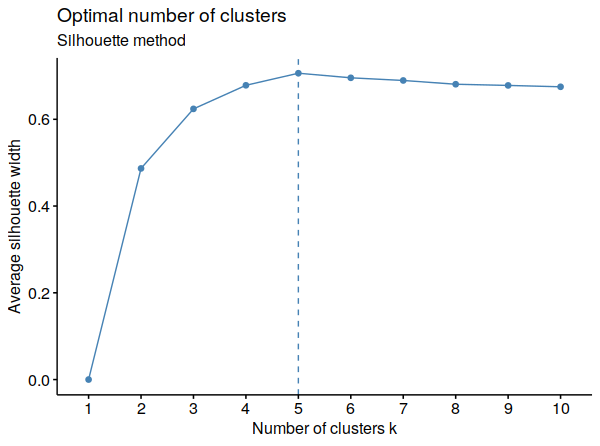
\includegraphics[scale=.5]{images/clusterSilhouette.png} 
	\label{i_cluster_Silhouette}
	\caption{Silhouette promedio vs número de clusters}
\end{figure}

\pagebreak
\subsection{Asignación de clusters}

Habiendo elegido el número de clústers por crear, se procedió a calcular la asignación de los datos a cada clúster, usando clustering jerárquico con la ayuda de la función \textsf{agnes}. Los clústers obtenidos se muestran en las representaciones en dos dimensiones de los datos (PCA y Factores) en las figuras \ref{i_cluster_PCA} y \ref{i_cluster_Factores}. En ambos casos se observa que los grupos formados coinciden con los descritos en la sección de reducción de dimensión. Hay que notar que cada una de las marcas de pizza está contenida en un único clúster.

\begin{figure}[h]
\centering
	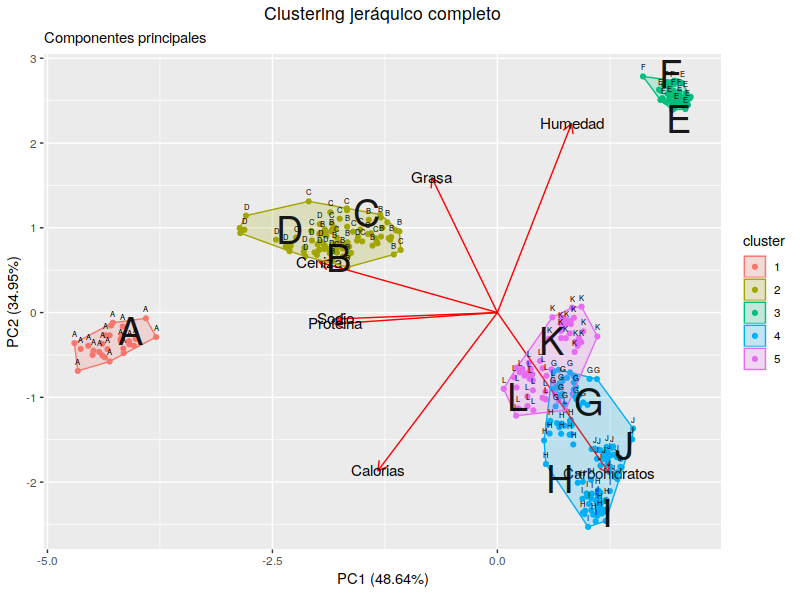
\includegraphics[scale=.75]{images/clusterPCA.png} 
	\label{i_cluster_PCA}
	\caption{Clustering jerárquico completo (Representación: PCA)}
\end{figure}


\begin{figure}[h]
\centering
	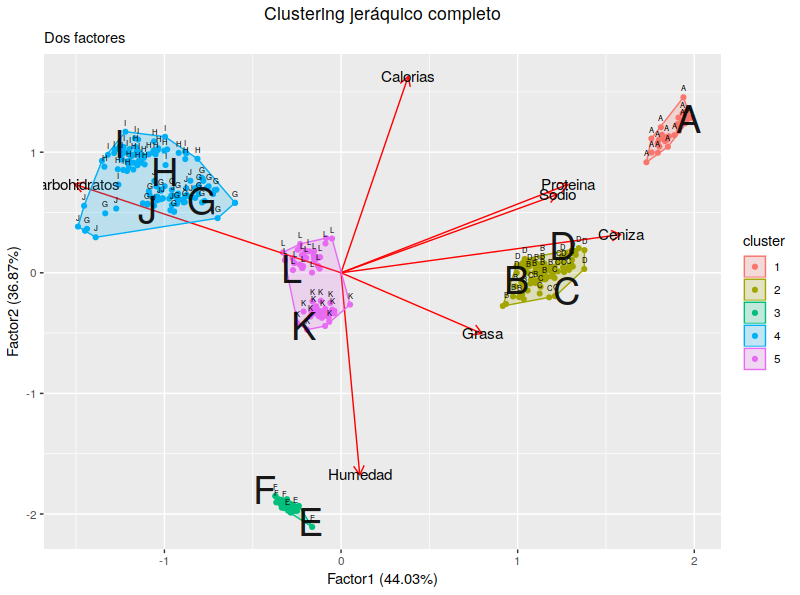
\includegraphics[scale=.75]{images/clusterFactores.png} 
	\label{i_cluster_Factores}
	\caption{Clustering jerárquico completo (Representación: Factores)}
\end{figure} 
\section{Modelos de clasificación.}

\section{Conclusiones.}



\end{document}